% Opciones empleadas:
%
%	a4paper -> indica el tama�o del papel, en este caso A4.
%	11pt -> tama�o de la fuente 11 puntos.
%	oneside -> s�lo escribimos en una cara del folio.
% 
% Otras opciones interesantes:
%
%	twoside -> escribimos a doble cara.
%	openbib -> para que las referencias bibliogr�ficas tengan un salto de l�nea entre cada campo de la referencia.
%
\documentclass[a4paper,11pt,twoside]{book}

% codificaci�n latin1 y s�mbolos del idioma espa�ol (�, acentos, ...)
\usepackage[english]{babel}
\usepackage[latin1]{inputenc}

% puede que queramos usar el s�mbolo del euro.
\usepackage{eurosym}

% El paquete fancybox nos permite crear cajas de diferentes estilos con facilidad.
% http://www.ctan.org/get/macros/latex/contrib/fancybox/fancybox.pdf
% http://www.mackichan.com/index.html?techtalk/487.htm~mainFrame
\usepackage{fancybox}
\usepackage{multicol}
\usepackage{amsmath}

% Para incluir subfiguras.
\usepackage{subfigure}

% Para incluir gr�ficos en JPG => compilar con pdflatex.
% \usepackage[pdftex]{graphicx}
\usepackage[pdftex]{graphicx}   % --> LaTex =>PDF con epstodf
\usepackage{epstopdf}

% Para incluir gr�ficos EPS => compilar con latex.
%\usepackage[dvips]{graphicx}

% Para escribir en color...
%
% ... cuando compilamos con el comando ``latex''
%\usepackage[dvips,usenames]{color}
% ... uando compilamos con el comando ``pdflatex''
\usepackage[pdftex,usenames,dvipsnames]{color}

% Espaciado y ajuste de m�rgenes
\usepackage{setspace}
\onehalfspacing
% \doublespacing
\setlength{\textwidth}{15cm}
\setlength{\textheight}{22cm}
\setlength{\oddsidemargin}{1cm}
\setlength{\evensidemargin}{1cm}
%\usepackage[hmargin={4cm,2.5cm},tmargin=4cm,bmargin=4cm]{geometry}
%Code snippets.
\usepackage{listings}
%Landscape figures.
\usepackage{lscape}

% Paquete fancyhdr -> Para modificar la cabecera y pie de p�ginas.
% http://tug.ctan.org/tex-archive/macros/latex/contrib/fancyhdr/
\usepackage{fancyhdr}
\pagestyle{fancy}
\fancyhf{}
\fancyhf[HR]{\thepage}
\fancyhf[HL]{\nouppercase\rightmark}

% Package booktabs -> Para mejorar el aspecto de las tablas o cuadros.
% http://www.ctan.org/tex-archive/macros/latex/contrib/booktabs/
\usepackage{booktabs}
\usepackage[pagebackref=true, hypertexnames=true]{hyperref}
% Package rotating -> Para poder girar las tablas y dibujarlas a lo largo
% del folio en vez de a lo ancho.
\usepackage{rotating}

% Packages multicol y multirow, para manejar tablas de filas y columnas m�ltiples.
\usepackage{multicol}
\usepackage{multirow}
%To center the captions.
\usepackage[center]{caption}

%Links in biblio.
\usepackage{url}

% Personalizamos la separaci�n entre p�rrafos...
\parskip=6pt

% Personalizamos el identado en la primera l�nea del nuevo p�rrafo...
\parindent=0pt

% Establecemos el n�mero m�ximo de niveles de profundidad en las secciones.
\setcounter{secnumdepth}{3}

% T�tulo
\title{Global illumination for point based rendering}
% Autor
\author{Luis Omar Alvarez Mures}
% Fecha
\date{\today}


\begin{document}

	% \maketitle sirve para generar autom�tica una portada predefinida, pero para un proyecto fin de carrera
	%	de FIC no sirvir�a porque no cumple las normas de presentaci�n. Podemos hacer dos cosas:
	% 1. Usarla e ignorar las normas (y asumir las consecuencias que pueda tener)
	% 2. Hacernos una portada en LaTeX que cumpla las normas (menos arriesgado)
	%
        %
% Portada.
%

% Nota: Ser�a m�s c�modo emplear el comando \maketitle que genera una portada de forma autom�tica, pero 
% no incluye toda la informaci�n que es necesario incluir en la memoria de un proyecto de fin de carrera
% de la Facultad de Inform�tica de A Coru�a.
%

\begin{titlepage}

	\begin{center}

		% Logotipo de la universidad.
		
\includegraphics[width=6cm]{eps/00.eps}
		\vspace{2cm}

		% Nombre de la facultad, de la universidad y del departamento en que se realiza el PFC.
		{\Large{\textbf{Faculty of Computer Science}}}
		\\
		{\Large{\textbf{University of A Coru�a}}}
		\vspace{1cm}

		% Indicamos el nombre de la titulaci�n oficial que hemos cursado con tanto esfuerzo.
		{\large FINAL YEAR PROJECT\\COMPUTER SCIENCE DEGREE}
		\vspace{1cm}

		% T�tulo
		\textbf{\LARGE Real-time management tool for massive 3D point clouds}
		\vspace{7cm}
	\end{center}

	\begin{flushright}
		\begin{tabular}{ll}
			% Nombre del alumno.
			\large{\textbf{Student:}}	&
			\large{Luis Omar Alvarez Mures} \\

			% Nombre del director/tutor del proyecto.
			\large{\textbf{Advisors:}}	&
			\large{Emilio Jos� Padr�n Gonz�lez} \\
			 & \large{Alberto Jaspe Villanueva} \\

			% Fecha.
			\large{\textbf{Date:}}	&
			\large{\today} \\
		\end{tabular}
	\end{flushright}

\end{titlepage}

        \thispagestyle{empty}
        \cleardoublepage
        %\newpage
	%\thispagestyle{empty}
	%\mbox{}

	% FRONTMATTER: TOC, LOF, LOT y descripci�n/organizaci�n de la memoria.
        \frontmatter
	
	% Los proyectos de fin de carrera de FIC han de ir acompa�ados de una serie de documentos adicionales, algunos
	% 	de ellos obligatorios (certificado, resumen, lista de palabras clave) y otros opcionales (dedicatoria
	%	y agradecimientos).
	%
	
        %\thispagestyle{empty}     % No number page, headings...
        %%
% Certificado
%

\begin{center}
	\begin{minipage}[t][6cm][l]{.8\textwidth}
		\begin{center}
			% Nombre del director del proyecto
			D. {\sc Nombre Del Director del Proyecto}

			% A los profesores les gusta que se indique su grado o posici�n en la estructura de la universidad :-P
			Profesor de Escuela o Facultad Universitaria

			% Departamento al que pertenece el director y en el que se realiza el proyecto.
			Departamento de lo que sea

			Universidad de A Coru�a
		\end{center}
	\end{minipage}
\end{center}

% El director certifica que el proyecto obra de su proyectando constituye su Proyecto de Fin de Carrera en la titulaci�n indicada.
CERTIFICA:
Que la memoria titulada {\it ``Real-time management tool for massive 3D point clouds''} ha sido realizada por {\sc Luis Omar Alvarez Mures} bajo mi direcci�n y constituye su Proyecto de Fin de Carrera de Nombre de la Titulaci�n Que Corresponda.

\vspace{5cm}

En A Coru�a, a \today

% Espacio para que pueda firmar el certificado que debe acompa�ar al proyecto.
\vspace{3cm}

\begin{center}
	\begin{minipage}[t][4cm][l]{.5\textwidth}
	% Nombre del director del proyecto
	D. {\sc Nombre Del Director del Proyecto}
	\\
	Director del proyecto
	\end{minipage}
\end{center}

        
        \thispagestyle{empty}     % No number page, headings...
	\vspace*{\fill}

\begin{center}
	\begin{tabular}{ll}
		% Nombre del alumno.
		\large{\textbf{T�tulo:}}	&
		\large{Ferramenta para o traballo interactivo con grandes nubes de puntos 3D} \\
		\\
		% Nombre del director/tutor del proyecto.
		\large{\textbf{Clase:}}	&
		\large{Proxecto de desenvolvemento en investigaci�n} \\
		\\
		% Fecha.
		\large{\textbf{Autor:}}	&
		\large{Luis Omar Alvarez Mures} \\
		\\
		\large{\textbf{Directores:}}	&
		\large{Alberto Jaspe Villanueva} \\
		& \large{Emilio Jos� Padr�n Gonz�lez} \\
		\\
		\large{\textbf{Tribunal:}}	&
		\large{Emilio Jos� Padr�n Gonz�lez} \\
		& \large{Guillermo L�pez Taboada} \\
		& \large{Jos� Rodrigo Sanjurjo Amado} \\
		\\
		\large{\textbf{Data de lectura:}}	&
		\large{9 de xullo, 2012} \\
		\\
		\large{\textbf{Cualificaci�n:}}	&
		\large{} \\
	\end{tabular}
\end{center}

\vspace*{\fill}

	
	\thispagestyle{empty}
        \cleardoublepage
	
	\thispagestyle{empty}     % No number page, headings...
	%
% Dedicatoria
%
\section*{}

\begin{flushright}
	{\it Dedicated to Rebeca and my parents.}
\end{flushright}

        
        \thispagestyle{empty}
        \cleardoublepage
        
        %\newpage
	%\thispagestyle{empty}
	%\mbox{}
	
	\thispagestyle{empty}
        %
% Agradecimientos
%

\section*{Acknowledgements\footnote{In alphabetical order}}

My sincerest thank you for the help provided:

To Mr. Alberto Jaspe Villanueva.

To Mr. Emilio Jos� Padr�n Gonz�lez.

To Mr. Juan Ram�n Rabu�al Dopico.




        
        \thispagestyle{empty}
        \cleardoublepage
        %\newpage
	%\thispagestyle{empty}
	%\mbox{}
	
	\thispagestyle{empty}
        %
% Resumen del proyecto de fin de carrera
%

\section*{Resumo:}

O render baseado en puntos ten m�ltiples vantaxes respecto do cl�sico que utiliza mallas de pol�gonos, sobre todo no caso no que os pol�gonos poidan chegar a ser m�is pequenos ca un pixel.

O obxectivo deste proxecto � dese�ar e implementar un motor de render baseado en puntos que utilice raytracing como m�todo de iluminaci�n global. Ao ser un campo todav�a pouco explorado, o proxecto presenta unha importante compo�ente investigadora, xa que implica a b�squeda de soluci�ns que nos permitan resolver os distintos problemas que xurden nas diferentes fases dun \emph{pipeline} gr�fico para o render de puntos. Tres son as principais metas que se propuxeron acadar con este proxecto:
\begin{itemize}
\item Desenvolver un motor de \emph{ray tracing} desde cero.
\item Investigar como as t�cnicas de iluminaci�n global m�is habituais poden ser aplicadas en render baseado en puntos.
\item Comprobar o potencial do punto como primitiva gr�fica dun motor de render.
\end{itemize}

O motor proposto segue un dese�o totalmente modular, con varias etapas
que permiten desacoplar as distintas operaci�ns a realizar para obter o render dunha escena 3D. As�, primeiro precisaremos gardar a informaci�n que o motor necesita para renderizar unha escea (cousas coma a posici�n da c�mara, orientaci�n, etc.). Para iso util�zase un arquivo de configuraci�n XML que cont�n todos estos datos, as� como calquera outra informaci�n relevante para o proceso de render.

Seguidamente prec�sase gardar os datos da nube de puntos. Para iso � necesario saber a posici�n, vector normal, etc. de cada punto, para o que utilizamos un arquivo de texto ASCII que cont�n toda a informaci�n da escena de entrada e que ademais soporta control de versi�ns, permitindo cambios no formato. Tam�n ofreceremos unha interfaz integrada en Blender que permite ao usuario crear datasets en Blender e renderizarlos co noso motor. Isto dota � proxecto dunha gran flexibilidade, xa que � capaz de renderizar datasets ou calquer escea en Blender.

Despois deste paso, prec�sase elexir o modelo de c�mara a usar. No noso motor implementamos d�as opci�ns diferentes. As�, � posible elexir entre unha c�mara axonom�trica ou en perspectiva (dependendo do modo de render elexido). Por outra banda, tam�n � posible elexir entre obter o render mediante a proxecci�n da escena na c�mara ou ben usando raytracing. A�nda que o motor implementa ambas alternativas, concentrar�monos no raytracing, posto que � a opci�n que m�is posibilidades e prestaci�ns ofrece, sendo o caso a estudar no proxecto.

� importante rese�ar que debido � natureza das nubes de puntos, que tenden a ter unha gran cantidade de datos, para a aceleraci�n do proceso de raytracing o motor permite utilizar unha estrutura de aceleraci�n espacial que permita organizar as nubes de puntos para optimizar determinadas operaci�ns cos mesmos (intersecci�n raio-escena, b�squeda de veci�os, etc.). Concretamente, neste proxecto implementouse un k-d tree como estrutura de aceleraci�n. O uso do k-d tree permite obter unha importante mellora no rendemento do noso motor.

Respecto ao tradicional render baseado en pol�gonos, o render con puntos presenta algunhas desvantaxes, como por exemplo a natureza adimensional dos mesmos. Isto quere dicir que o punto non ten superficie, volumen ou normal, o que introduce novos problemas en moitas das operaci�ns com�ns dun motor de render: intersecci�ns, iluminaci�n, etc. Concretamente, no caso do c�lculo da iluminaci�n � imprescindible dispor dos vectores normais �s distintas superficies da escena, neste caso representadas por puntos. Se non se disp�n destas normais, � necesario estimalas dalg�n xeito. Para resolver este problema o proxecto utiliza un m�todo de m�nimos cadrados que se usa para estimar a normal nun punto dependendo de donde est�n os seus veci�os.

A derradeira etapa do noso motor, pero non menos importante de acordo aos obxectivos do proxecto, � a iluminaci�n da escena. O motor ofrece d�as opci�ns. Por un lado p�dese utilizar un m�todo de \emph{hard shadows}, menos custoso computacionalmente pero con resultados pouco realistas. Por outra banda,
o motor implementa o m�todo de \emph{Monte Carlo}, modelo de iluminaci�n global que trata de simular o comportamento real da luz nun contorno, ofrecendo resultados m�is realistas, a�nda que significativamente m�is custosos.

Posto que o motor fai un importante uso de distintas operaci�ns e funci�ns matem�ticas ao longo de todas as s�as fases, o proxecto tam�n incorpora unha librer�a matem�tica que se encarga destas tarefas.



        
        \thispagestyle{empty}
        \cleardoublepage
	
	\thispagestyle{empty}
        %
% Resumen del proyecto de fin de carrera
%

\section*{Abstract:}

The objective of this project is designing and implementing a point-based rendering engine that utilizes ray tracing for global illumination computation. 

Point-based rendering has several advantages compared to the more classic polygon-based rendering that uses polygon meshes, specially when polygons can be smaller than a pixel.

In this project we explore how to represent point models without ray tracing techniques (with a projective camera) and using ray tracing that is the true focus of this project.

It is also important to mention that because of the nature of point clouds, datasets tend to be really large. That is why a k-d tree is used to accelerate the ray tracing process. A k-d tree is a space partitioning structure for data organization (in our case, point data). This acceleration structure reduces greatly rendering times, and without it the rendering process would take too long and be too computationally expensive.

Point-based rendering also has some disadvantages, like for example the zero-dimensional nature of points. This means that a point has no surface, volume or normal vector. This results in problems in the rendering process. In this project we explore several solutions for these problems.

To facilitate the usage of the project to the end user, and to also make testing easier; a plugin compatible with Blender will be programmed. It allows the rendering of scenes created in Blender with our project and facilitates the use of the engine thanks to the integration with the interface of Blender. 



        
        \thispagestyle{empty}
        \cleardoublepage
        
        \thispagestyle{empty}     % No number page, headings...
	%\include{pfc_palabras_clave}
	
	\thispagestyle{empty}
        \cleardoublepage
	
        \thispagestyle{empty}     % No number page, headings...
        %\include{pfc_soft_hard}
        
        \thispagestyle{empty}
        \cleardoublepage
        
       % \thispagestyle{empty}     % No number page, headings...
        
        %\newpage
	%\thispagestyle{empty}
	%\mbox{}

        \tableofcontents
        \listoffigures
        \listoftables
        
        %\newpage
	%\thispagestyle{empty}
	%\mbox{}

	% MAINMATTER: El contenido, cap�tulo a cap�tulo, de la memoria del PFC.
        \mainmatter

	%
% Frontmatter - Introducci�n. Los miembros del tribunal que juzgan los PFC's tienen muchas m�s memorias que leer, por lo que
%	agradecer�n cualquier detalle que permita facilitarles la vida. En este sentido, realizar una peque�a introducci�n,
%	comentar la organizaci�n y estructura de la memoria y resumir brevemente cada cap�tulo puede ser una buena pr�ctica
%	que permita al lector centrarse f�cilmente en la parte que m�s le interesa.
%

\chapter[Introduction]{
	Introduction
}

Computer Graphics is a discipline that creates graphics using a computer. Advances in computer graphics have had an impact on several media types such as for example, the movies and video games industry, civil engineering, etc.

Images are normally captured by optical devices; such as cameras, LIDAR, mirrors, lenses, etc. Rendering is the process of generating an image from a model, the \emph{scene}, by means of a computer. A scene contains information like geometry, lighting, etc. about a virtual scene.

Typically, polygonal modeling has been the approach followed for modeling objects in the scene, approximating their surfaces using polygons. Point-based graphics focuses on points as the fundamental representation of the surfaces instead of polygons (see \figurename~\ref{poly_comp}).

\begin{figure}[h]
	\centering
	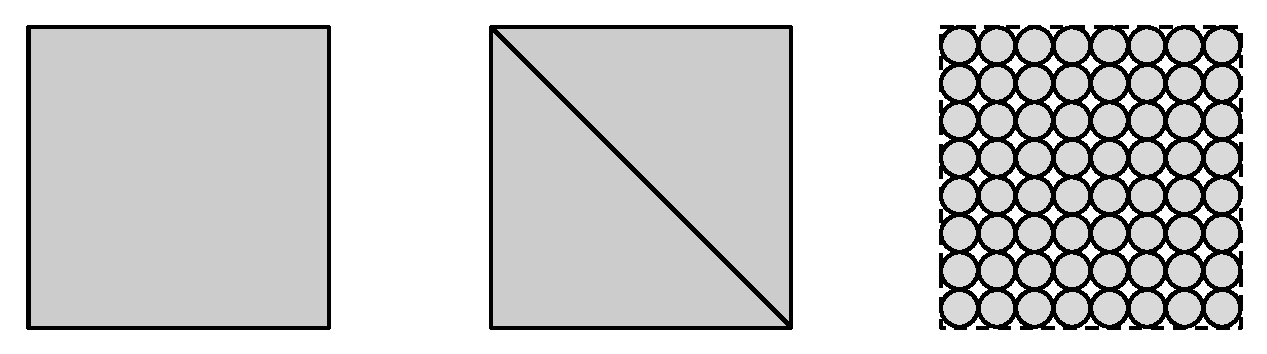
\includegraphics[scale=0.6]{eps/pol_comp.pdf}
	\caption[Modeling types comparison]{
		From left to right; mathematical representation of a plane, representation using two polygons (triangles) and a point-based representation.
	}
	\label{poly_comp}
\end{figure}

Using point based representations, the polygonal approximation step can be skipped and the massive amount of captured data is directly used.

All of these concepts will be explained in depth in their corresponding chapters. 

\section[Motivation and context]{
	Project motivation and context
}

Lately, 3D acquisition systems (commonly known as LIDAR\footnote{\textit{Laser Imaging Detection And Ranging}}) have evolved causing a revolution in work methodologies of several disciplines, from civil engineering, architecture, cultural heritage, movies to videogames. These systems use ultraviolet, visible or near infrared light to image objects. It can target a wide range of materials and even single molecules. A narrow laser beam can map features with very high precision.

Each sample obtained will possess coordinates (x,y,z), color, normal, temperature, etc. This information can be used to obtain measurements, calculations, etc. without having to repeat the capture process again each time we want to measure something new already present in the dataset. This presents clear advantages compared to the classical work-flow of a topographer that would have to measure on site each time a new measurement is required.       

PCM \cite{PCM} is a software library developed by the UDC\footnote{\textit{University of A Coru�a}} for the management of big point datasets obtained using LIDAR. PCM includes basic memory hierarchy management, making it possible to transfer the point cloud data between secondary memory (HDD) and video memory in the graphics card. PCM includes a very basic visualizer, that has the potential to become the seed for a more advanced point cloud software tool that will allow the user to access all of these features in real-time.   

Because of the massive nature of these datasets (some of them possess more than a billion points) achieving real-time manipulation of them is a complex task. It will require the improvement of PCM and a careful performance analysis. Having a system that is able to deal with these amounts of data, will let the user take advantage of the full precision of the capture devices if needed. 

Also because of the huge amounts of data, the possibility of using the massive parallel computing power of graphics cards will be explored. The large number of parallel processors can be used to reduce the computation times as much as possible. 

In this project, a complete software tool for visualization, management and manipulation of massive 3D point clouds will be developed. The tool will be multiplatform (GNU/Linux, Windows and MacOS) and will make use of open source software. That is why for the user interface it will take advantage of QT, that has native tools for all the aforementioned platforms. The resulting QT application will let the user access all of the functionality including an advanced and complete 3D visualizer.
   

\section[Objetives]{
	Project objetives
}

The aim of this project is the design and implementation of a point-based multiplatform software tool for interactive visualization, management and manipulation of massive 3D point clouds. 

The application will offer the user the necessary tools to work effectively with this type of datasets, including a 3D visualizer with advanced point-rendering techniques using OpenGL, that will allow real time interaction with one or multiple point clouds. 

From the interface, the user will be able to:     

\begin{itemize}
\item Select different visualization modes for point-based models: multiple cameras, simple and advanced visualization, multi-resolution, etc.
\item Combine different point clouds with tools that enable rotation, translation and scaling of the clouds.
\item Select points in the clouds for working with them.
\item Apply operations to a part of the cloud or the complete dataset. From simple operations like distance measurements to plane or other geometric primitives detection.
\item Export the work done to a standard CAD format, so the tool can be integrated in other workflows. 
\end{itemize}

The developed tool will take advantage of the parallel computing possibilities of the platforms. Either using the GPGPU capabilities of the graphics card with OpenCL or the multiple cores of the CPU. 

PCM will be used as the foundation for this work. PCM is a project in development that offers several low level tools for working with point clouds of arbitrary size in commodity hardware, from which a multi-resolution structure with different levels of cache is highlighted. This final year project will not only extend PCM with the mentioned features, offering a high level tool for the final user, but will also improve the existing source code; paying special attention to performance aspects.

\section[Structure]{
Document structure
}

 





	%\include{pfc_main_070}
	%\include{pfc_main_000}
	%\include{pfc_main_010}
	%\include{pfc_main_020}
	%\include{pfc_main_030}
	%\include{pfc_main_040}
	%\include{pfc_main_050}
	%\include{pfc_main_060}
	%\include{pfc_main_080}

	% INCLUIMOS LOS AP�NDICES...
        %\appendix
	%\include{pfc_appendix_010}
%         \include{pfc_appendix_020}

	%Primero hay que compilar el bibtex para que salga.
	% INCLUIMOS LA BIBLIOGRAF�A...
	\nocite{*}	% Se usa para indicar en la bibliograf�a las referencias no citadas.
	\bibliography{pfc_biblio}
	\bibliographystyle{alpha}

\end{document}

